As \emph{link-cut trees} são uma estrutura de dados usada para dar suporte a operações sobre florestas enraizadas~\cite{DemaineHJSI2012}.  

Em nossa aplicação, queremos utilizá-las para manipular florestas simples (não enraizadas). Para isso, teremos que acrescentar à biblioteca
básica das \emph{link-cut trees} uma operação extra.  

Começaremos descrevendo a biblioteca básica, voltada a florestas enraizadas~\cite{RamchandraCODEFORCE}. A interface básica neste caso contém as seguintes rotinas:  

\begin{itemize}
    \item \texttt{maketree()}: cria uma árvore enraizada com um único nó e o devolve.  

    \item \texttt{link(Node u, Node v)}: recebe um nó \texttt{u} que é raiz de uma árvore enraizada e um nó \texttt{v} de uma outra árvore enraizada e adiciona o arco de \texttt{u} para \texttt{v} juntando as duas árvores enraizadas.

    \item \texttt{cut(Node v)}: recebe um nó \texttt{v} de uma árvore enraizada em que \texttt{v} não é a raiz e remove o arco de \texttt{v} para seu pai na árvore, resultando em duas árvores enraizadas: uma com \texttt{v} e seus descendentes e outra com os demais nós da árvore enraizada original de \texttt{v}.

    \item \texttt{findroot(Node u)}: recebe um nó \texttt{u} de uma árvore enraizada e devolve a raiz da árvore.
\end{itemize}

Para manipular florestas simples, não enraizadas, adicionamos à interface uma rotina que altera a raiz de uma árvore enraizada para um outro nó arbitrário da árvore:  

\begin{itemize}
    \item \texttt{evert(Node v)}: recebe um nó \texttt{v} de uma árvore enraizada e modifica a árvore tornado \texttt{v} a raiz da árvore. Mais precisamente, inverte a orientação dos arcos no caminho de \texttt{v} até a raiz da árvore em que \texttt{v} se encontra.
\end{itemize}

Essa biblioteca de funções pode ser implementada por meio de \emph{splay trees}, de modo que o consumo de tempo do \texttt{maketree} seja $\Oh(1)$, e o consumo de tempo do \texttt{link}, \texttt{cut}, \texttt{findroot} e \texttt{evert} seja $\Oh(\lg n)$ amortizado por operação, onde $n$ é o número de chamadas a \texttt{maketree}.  

Para implementar as rotinas das \emph{link-cut trees} eficientemente, mantemos para cada nó da floresta o chamado filho preferido do momento: cada nó rastreia o filho que foi acessado por último nas operações executadas na floresta. O nó mais profundo acessado fica sem filho preferencial. Essa informação particiona cada árvore da floresta nos chamados caminhos preferenciais. Veja o exemplo da Figura~\ref{fig:lct}(a).  

\begin{figure}[htb]
    \centering
    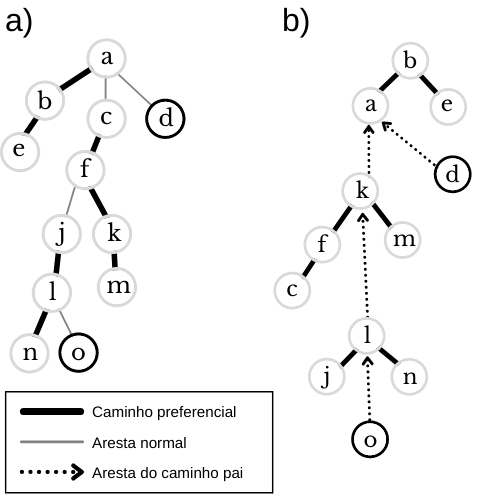
\includegraphics[width=8cm]{lct-and-represented-tree2.png}
    \caption{Exemplo de link-cut tree.}\label{fig:lct}
\end{figure}

A implementação mantém os nós de cada caminho preferencial em uma \emph{splay tree}, considerando a profundidade do nó no caminho como a chave (implícita).  
As várias \emph{splay trees} dos caminhos preferenciais de uma mesma árvore enraizada estão organizadas de acordo com os arcos da floresta que ligam estes caminhos. Veja a Figura~\ref{fig:lct}(b).  

A operação \texttt{maketree} simplesmente aciona a operação \texttt{makeSplay}. Para descrever o funcionamento das operações \texttt{link}, \texttt{cut}, \texttt{findroot} e \texttt{evert}, utilizamos a seguinte operação interna das \emph{link-cut trees}:  

\begin{itemize}
    \item \texttt{access(Node v)}: reorganiza os caminhos preferenciais estabelecendo \texttt{v} e cada ascendente de \texttt{v} como filho preferido de seu pai, e deixando \texttt{v} sem filho preferencial. Veja um exemplo do efeito da operação \texttt{access} na Figura~\ref{fig:access}.  
\end{itemize}


\begin{figure}[htb]
    \centering
    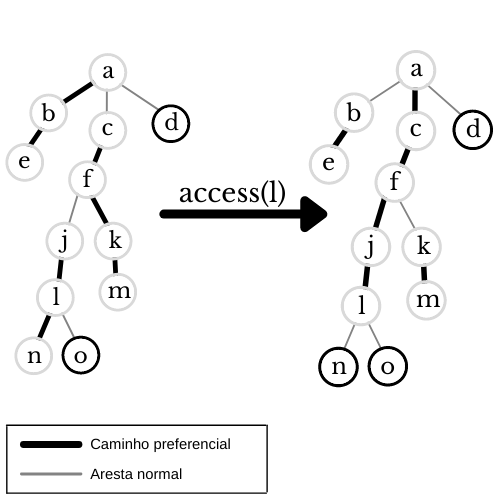
\includegraphics[width=8cm]{figura2.png}
    \caption{Exemplo da operação \texttt{access}.}
    \label{fig:access}
\end{figure}


Com essa operação, conseguimos descrever as operações \texttt{link}, \texttt{cut} e \texttt{evert} em termos das operações das \emph{splay trees}.  

No \texttt{link(u, v)}, acionamos o \texttt{access}~\cite{wiki:LinkCutTree} em \texttt{u} e em \texttt{v}, e depois acionamos um \texttt{join} das \emph{splay trees} dos caminhos preferenciais de \texttt{u} e de \texttt{v}.  

No \texttt{cut(v)}, acionamos o \texttt{access} em \texttt{v} e o \texttt{split} no predecessor do \texttt{v} na \emph{splay tree} do seu caminho preferencial.  

No \texttt{evert(v)}, acionamos o \texttt{access} em \texttt{v} e em seguida o \texttt{reflect} na \emph{splay tree} do caminho preferencial de \texttt{v}.  

A operação \texttt{access} é a mais complexa, pois modifica várias das \emph{splay trees} que compõem a \emph{link-cut tree} de uma árvore enraizada. Devido tal complexidade, decidimos, nesse relatório, por omitir a descrição dessa operação em termos das operações das \emph{splay trees}.  

